\documentclass[a4paper,showframe,11pt]{report}\usepackage[]{graphicx}\usepackage[]{color}
%% maxwidth is the original width if it is less than linewidth
%% otherwise use linewidth (to make sure the graphics do not exceed the margin)
\makeatletter
\def\maxwidth{ %
  \ifdim\Gin@nat@width>\linewidth
    \linewidth
  \else
    \Gin@nat@width
  \fi
}
\makeatother

\definecolor{fgcolor}{rgb}{0.196, 0.196, 0.196}
\newcommand{\hlnum}[1]{\textcolor[rgb]{0.063,0.58,0.627}{#1}}%
\newcommand{\hlstr}[1]{\textcolor[rgb]{0.063,0.58,0.627}{#1}}%
\newcommand{\hlcom}[1]{\textcolor[rgb]{0.588,0.588,0.588}{#1}}%
\newcommand{\hlopt}[1]{\textcolor[rgb]{0.196,0.196,0.196}{#1}}%
\newcommand{\hlstd}[1]{\textcolor[rgb]{0.196,0.196,0.196}{#1}}%
\newcommand{\hlkwa}[1]{\textcolor[rgb]{0.231,0.416,0.784}{#1}}%
\newcommand{\hlkwb}[1]{\textcolor[rgb]{0.627,0,0.314}{#1}}%
\newcommand{\hlkwc}[1]{\textcolor[rgb]{0,0.631,0.314}{#1}}%
\newcommand{\hlkwd}[1]{\textcolor[rgb]{0.78,0.227,0.412}{#1}}%
\let\hlipl\hlkwb

\usepackage{framed}
\makeatletter
\newenvironment{kframe}{%
 \def\at@end@of@kframe{}%
 \ifinner\ifhmode%
  \def\at@end@of@kframe{\end{minipage}}%
  \begin{minipage}{\columnwidth}%
 \fi\fi%
 \def\FrameCommand##1{\hskip\@totalleftmargin \hskip-\fboxsep
 \colorbox{shadecolor}{##1}\hskip-\fboxsep
     % There is no \\@totalrightmargin, so:
     \hskip-\linewidth \hskip-\@totalleftmargin \hskip\columnwidth}%
 \MakeFramed {\advance\hsize-\width
   \@totalleftmargin\z@ \linewidth\hsize
   \@setminipage}}%
 {\par\unskip\endMakeFramed%
 \at@end@of@kframe}
\makeatother

\definecolor{shadecolor}{rgb}{.97, .97, .97}
\definecolor{messagecolor}{rgb}{0, 0, 0}
\definecolor{warningcolor}{rgb}{1, 0, 1}
\definecolor{errorcolor}{rgb}{1, 0, 0}
\newenvironment{knitrout}{}{} % an empty environment to be redefined in TeX

\usepackage{alltt}
\usepackage{standalone}
\standalonetrue
\ifstandalone
  \usepackage{../../haziq_thesis}
  \usepackage{../../haziq_maths}
  \usepackage{../../haziq_glossary}
  \addbibresource{../../bib/haziq.bib}
  \externaldocument{../01/.texpadtmp/introduction}
\fi





\IfFileExists{upquote.sty}{\usepackage{upquote}}{}
\begin{document}

Data from 27 separate smoking cessation studies in which participants are subjected to a nicotine gum treatment or a placebo.
The interest is to estimate the treatment effect size, and whether it is statistically significant.
The studies are conducted at different times and due to various reasons such as funding and cultural effects, the results from all of the studies may not be in agreement.
The number of effective participants plays a major role in determining the power of the statistical tests performed in individual studies.
The question then becomes how do we meaningfully aggregate all the data to come up with one summary measure?

Several methods exist to analyse such data sets.
One may consider a fixed-effects model, similar to a one-way ANOVA model to establish whether or not the effect size is significant.
Because of the study-specific characteristics, it is natural to consider multilevel or random-effects models as a means to estimate the effect size.
Regardless of method, the approach of analysing study-level treatment effects instead of patient-level data is the paradigm for meta-analysis.
However, analysing study-level estimates of effect size can be problematic for various reasons, such as small group samples or rare occurences.
Our approach using I-priors looks at patient-level data, but takes into account the levels due to the various study groups.

\begin{knitrout}
\definecolor{shadecolor}{rgb}{1, 1, 1}\color{fgcolor}\begin{figure}

{\centering 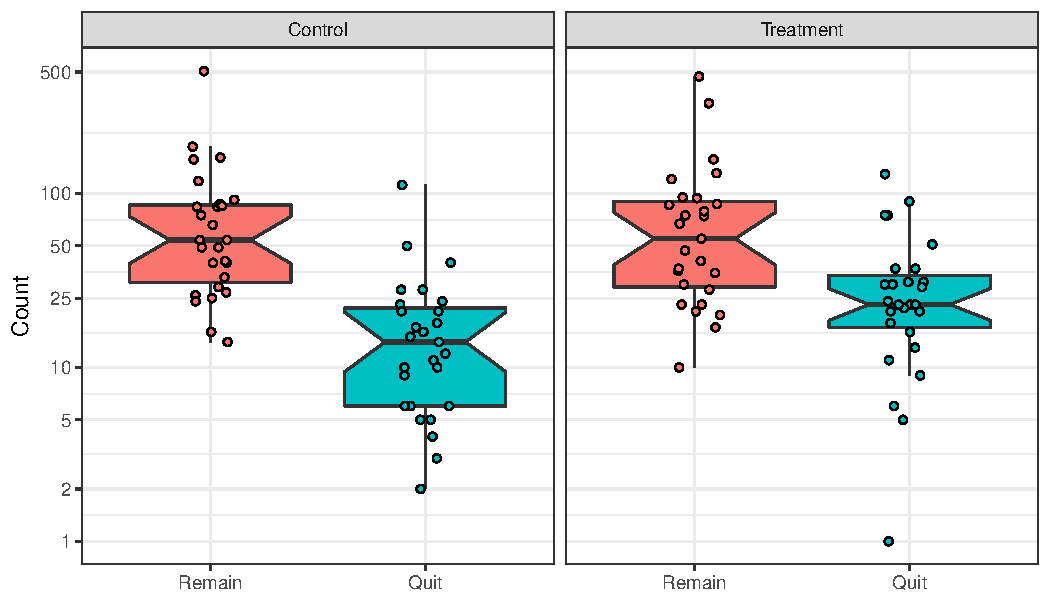
\includegraphics[width=\maxwidth]{figure/plot_data_smoke-1} 

}

\caption[Comparative box-plots of the distribution of patients who successfully quit smoking and those who remained smokers, in the two treatment groups]{Comparative box-plots of the distribution of patients who successfully quit smoking and those who remained smokers, in the two treatment groups.}\label{fig:plot.data.smoke}
\end{figure}


\end{knitrout}

A summary of the data is displayed by the box-plot in Figure \ref{fig:plot.data.smoke}.
On the whole, there are a total of 5908 patients, and they are distributed roughly equally among the control and treatment groups (46.33\% and 53.67\% respectively, on average).
From the box-plots, it is evident that there are more patients who quit smoking in the treatment group as compared to the placebo control group.
There are various measures of treatment effect size, such as risk ratio or risk differences, but we shall concentrate on \emph{odds ratios} as defined by
\[
  \text{odds ratio} = \frac{\text{odds of quitting smoking in \emph{treatment} group}}
  {\text{odds of quitting smoking in \emph{control} group}}.
\]
The odds of quitting smoking in either group is defined as
\[
  \text{odds} = \frac{\Prob[\text{quit smoking}]}{1 - \Prob[\text{quit smoking}]},
\]
and these probabilities, odds and ultimately the odds ratio can be estimated from sample proportions.
This raw odds ratio for all study groups is calculated as $1.66 = e^{0.50}$.
It is also common for the odds ratio to be reported on the log scale (usually as a remnant of logistic models).
A value greater than one for the odds ratio (or equivalently, greater than zero for the log-odds ratio) indicates a significant treatment effect.

A random-effects analysis using a multilevel logistic model has been considered by \hltodo{cite Skrondal Rabe-Hasketh, Agresti and Hartzel}.
Let $i=1,\dots,n_j$ index the patients in study group $j \in \{1,\dots,27\}$.
For patient $i$ in study $j$, $p_{ij}$ denotes the probability that the patient has successfully quit smoking.
Additionally, $x_{ij}$ is the centred dummy variable indicating patient $i$'s treatment group in study $j$.
These take on two values: 0.5 for treated patients and -0.5 for control patients.
The logistic random-effects model is
\begin{gather*}
  \log \left( \frac{p_{ij}}{1-p_{ij}} \right) = \beta_{0j} + \beta_{1j}x_{ij} \\
  \text{with} \\
  \begin{pmatrix} \beta_{0j} \\ \beta_{1j} \end{pmatrix}
  \sim \N \left(
  \begin{pmatrix} \beta_0 \\ \beta_1 \end{pmatrix},
  \begin{pmatrix} \sigma_0^2 & \sigma_{01} \\ \sigma_{01} & \sigma_1^2 \\ \end{pmatrix}
  \right)
\end{gather*}
Agresti also made the additional assumption that $\sigma_{01} = 0$ so that, coupled with the contrast coding used for $x_{ij}$, the total variance $\Var[\beta_{0j} + \beta_{1j}x_{ij}]$ would be constant in both treatment groups.
The overall log odds ratio is represented by $\beta_1$, and this is estimated as $0.57 = \log 1.76$.

In an I-prior model, the Bernoulli probabilities $p_{ij}$ are regressed against the treatment group indicators $x_{ij}$ and also the patients' study group $j$ via the regression function $f$ and a probit link:
\begin{align*}
  \Phi^{-1}(p_{ij})
  &= f(x_{ij}, j) \\
  &= f_1(x_{ij}) + f_2(j) + f_{12}(x_{ij}, j).
\end{align*}
We have decomposed our function $f$ into three parts: $f_1$ represents the treatment effect, $f_2$ represents the effect of the study groups, and $f_{12}$ represents the interaction effect between the treatment and study group on the modelled probabilities.
As both $x_{ij}$ and $j$ are nominal variables, the functions $f_1$ and $f_2$ both lie in the Pearson RKHS of functions $\cF_1$ and $\cF_2$, each with RKHS scale parameters $\lambda_1$ and $\lambda_2$.
As such, it does not matter how the $x_{ij}$ variables are coded (dummy coding 0, 1 vs. centred coding -0.5, 0.5) as the scaling of the function is determined by the RKHS scale parameters.
The interaction effect $f_{12}$ lies in the RKHS tensor product $\cF_1 \otimes \cF_2$.
In I-prior modelling, there are only two parameters to estimate, while in the standard logistic random-effects model, there are six. The results of the I-prior fit are summarised in the table below.


\begin{longtable}[t]{lrr>{\raggedleft\arraybackslash}p{2.4cm}}
\caption{\label{tab:mod.compare.smoke}Results of the I-prior model fit for three models.}\\
\toprule
Model & Lower bound & Brier score & No. of RKHS\newline scale param.\\
\midrule
$f_1$ & $-3210.76$ & 0.179 & 1\\
$f_1 + f_2$ & $-3092.22$ & 0.168 & 2\\
$f_1 + f_2 + f_{12}$ & $-3091.21$ & 0.168 & 2\\
\bottomrule
\end{longtable}



The approximated marginal log-likelihood value for the I-prior model (i.e. variational lower bound), the Brier score for each model and the number of RKHS scale parameters estimated in the model are reported in Table \ref{tab:mod.compare.smoke}. Three models were fitted: : 1) A model with only the treatment effect; 2) A model with a treatment effect and a study group effect; and 3) Model 2 with the additional assumption that treatment effect varies across study groups. Model 1 disregards the study group effects, while Model 2 assumes that the effectiveness of the nicotine gum treatment does not vary across study groups (akin to a varying-intercept model). Although not soundly based in theory, we may compare variational lower bounds of the three models for model selection as a proxy to using the true log-likelihood value. In this case, Model 3 has the highest lower bound value. The Brier score indicates the predictive performance of the models, and there is not much to distinguish between the three.

Unlike in the logistic random-effects model, where the log odds ratio can be read off directly from the coefficients, with an I-prior probit model the log odds ratio needs to be calculated manually from the fitted probabilities. The probabilities of interest are the probabilities of quitting smoking under each treatment group for each study group $j$ - call these $p_j(\text{treatment})$ and $p_j(\text{control})$. That is,
\begin{align*}
  p_j(\text{treatment}) &= \Phi\big( f(\text{treatment}, j) \big) \\
  p_j(\text{control})   &= \Phi\big( f(\text{control}, j) \big). \\
\end{align*}
The log odds ratio for each study group can then be calculated as usual.
For the overall log odds ratio, the probabilities that are used are the averaged probabilities weighted according to the sample sizes in each group. This has been calculated as $0.49 = \log 1.63$, slightly lower than both the raw log odds ratio and the log odds ratio estimated by the logistic random-effects model. This can perhaps be attributed to some shrinkage of the estimated probabilities due to placing a prior with zero mean on the regression functions.

\hltodo{RE: Fiona's suggestion of discussing the variance, covariance/correlation of the random effects?}

\begin{knitrout}
\definecolor{shadecolor}{rgb}{1, 1, 1}\color{fgcolor}\begin{figure}

{\centering 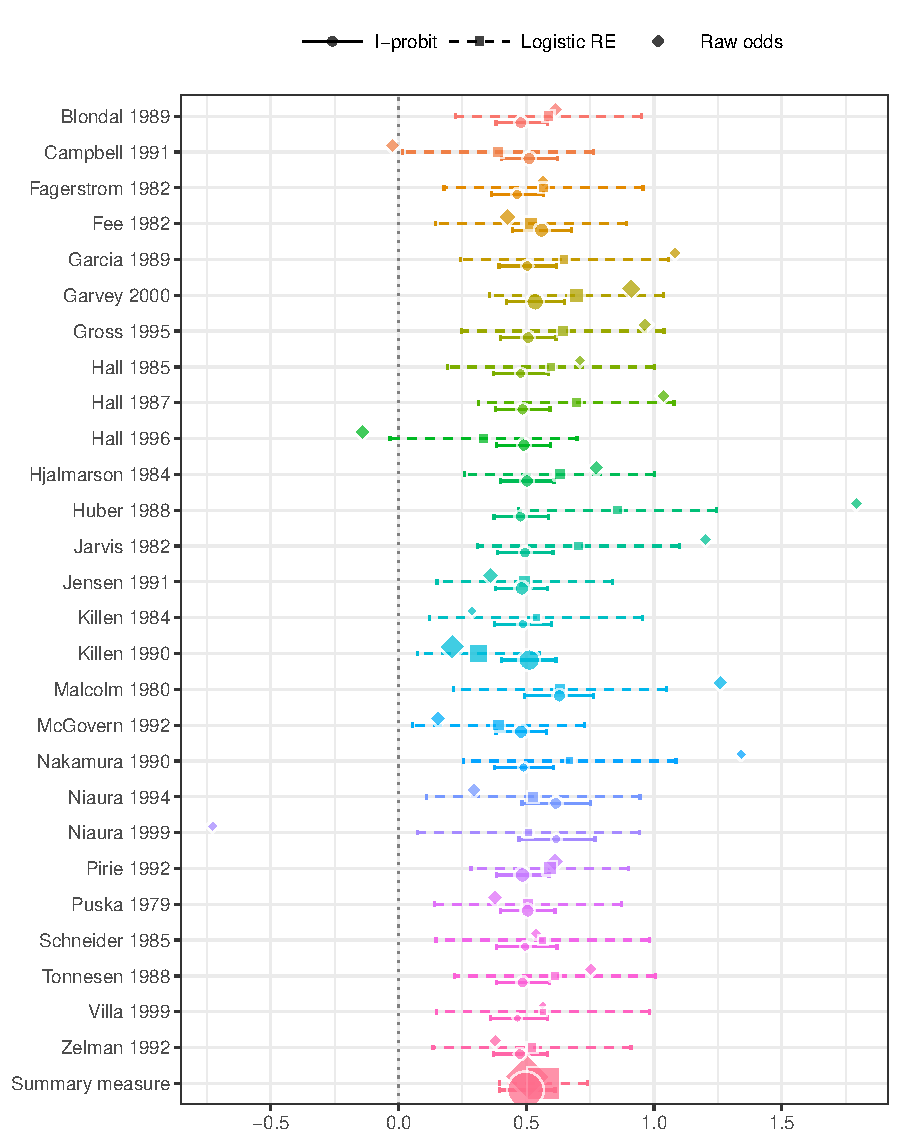
\includegraphics[width=\linewidth]{figure/smoke_forest_plot-1} 

}

\caption[Forest plot of effect sizes (log odds ratios) in each group as well as the overall effect size together with their 95\% confidence bands]{Forest plot of effect sizes (log odds ratios) in each group as well as the overall effect size together with their 95\% confidence bands. The plot compares the raw log odds ratios, the logistic random-effect estimates, and the I-prior estimates. Sizes of the points indicate the relative sample sizes per study group.}\label{fig:smoke.forest.plot}
\end{figure}


\end{knitrout}

\end{document}


